\documentclass[landscape]{slides}
\usepackage{color,graphicx,ifpdf,wasysym,type1cm}
\ifpdf
\DeclareGraphicsExtensions{.pdf,.png,.jpeg,.jpg}
\fi
\SetSymbolFont{operators}{normal}
                 {OT1}{cmr}{m}{n}
\SetSymbolFont{operators}{invisible}
                 {OT1}{cmr}{m}{In}
\definecolor{darkblue}{rgb}{0,0,0.5}
\definecolor{darkgreen}{rgb}{0,0.5,0}
\title{Command Line Slice Creation}
\author{Jonathon Duerig\\ University of Utah}
\date{20th July, 2010}
\newcommand{\heading}[1]{{\fontseries{b}\selectfont\begin{center}{\LARGE\color{red} #1}\end{center}}}
\newcommand{\code}[1]{\begin{center}{\tt #1}\end{center}}
\begin{document}
\fontfamily{cmr}\selectfont
\maketitle

\begin{slide}
\heading{Introduction}
\begin{small}
\begin{itemize}
\item The client machine
\item Your certificate passphrase
\item Checking your account
\item Slice registration
\item Sliver creation
\item Using your components
\item Cleaning up
\end{itemize}
\end{small}
\end{slide}

\begin{slide}
\heading{1. The client machine}
\begin{itemize}
\item The one you use!
\item It accesses GENI services via the Internet, and GENI resources via the
  control network.
\item In principle, just about any networked machine that can issue
  XMLRPC requests over HTTPS will do.
\item For today:
\code{users.emulab.net}
\end{itemize}
\end{slide}

\begin{slide}
\heading{Logging in with {\tt PuTTY}}
\begin{center}
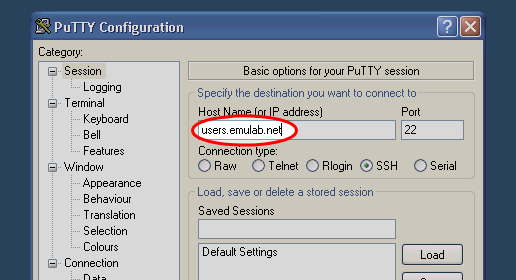
\includegraphics[width=17cm]{putty-1}
\end{center}
\end{slide}

\begin{slide}
\heading{Logging in with {\tt PuTTY}}
\begin{center}
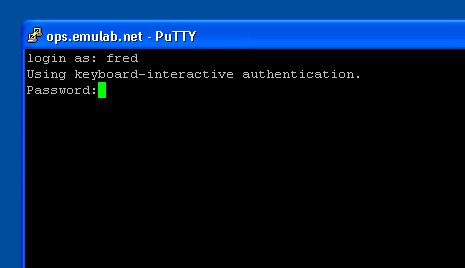
\includegraphics[width=17cm]{putty-2}
\end{center}
\end{slide}

\begin{slide}
\heading{Logging in with {\tt OpenSSH}}
\begin{center}
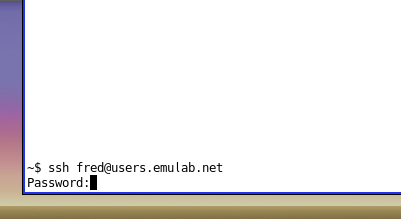
\includegraphics[width=17cm]{openssh}
\end{center}
\end{slide}

\begin{slide}
\heading{Getting to the scripts}
\begin{itemize}
\item On {\tt users.emulab.net}:
\end{itemize}
\begin{Large}\code{cd /proj/gec9tutorial/scripts}\end{Large}
\end{slide}

\begin{slide}
\heading{2. Store your passphrase}
\begin{itemize}
\item Your private key (matching your user certificate) is already
  on the client machine.
\item But it's passphrase protected...
\item You can either:
\begin{itemize}
 \item supply your passphrase for every script accessing the key
 \item or keep your passphrase in a plaintext file during a session (more
   convenient, but less secure).
\end{itemize}
\end{itemize}
\code{./rememberpassphrase.py}
\end{slide}

\begin{slide}
\heading{3. Inspect your account}
\begin{center}
\includegraphics[width=15cm]{tutorial-diagram-1}
\end{center}
\end{slide}

\begin{slide}
\heading{Inspect your account}
\begin{center}
\includegraphics[width=15cm]{tutorial-diagram-7}
\end{center}
\vspace{-4cm}
\begin{center}{\tt ./showuser.py }\emph{username}\end{center}
\end{slide}

\begin{slide}
\heading{4. Register a slice}
\begin{center}
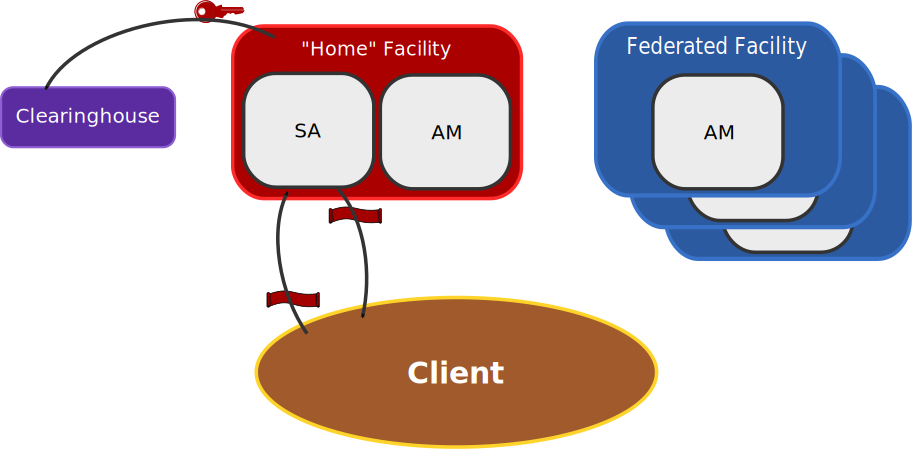
\includegraphics[width=15cm]{tutorial-diagram-2}
\end{center}
\vspace{-4cm}
\begin{center}{\tt ./registerslice.py -n }\emph{username}{\tt slice}\end{center}
\end{slide}

\begin{slide}
\heading{5. Inspect your account (again)}
\begin{center}
\includegraphics[width=15cm]{tutorial-diagram-7}
\end{center}
\vspace{-4cm}
\begin{center}{\tt ./showuser.py }\emph{username}\end{center}
\end{slide}

\begin{slide}
\heading{6. Create a sliver}
\begin{center}
\includegraphics[width=15cm]{slice}
\end{center}
\end{slide}

\begin{slide}
\heading{Create a sliver}
\begin{center}
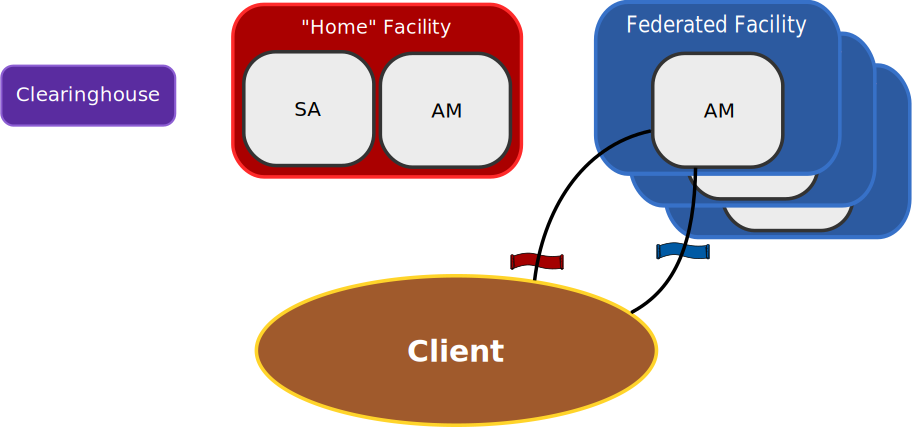
\includegraphics[width=15cm]{tutorial-diagram-5}
\end{center}
\vspace{-4cm}
\begin{center}{\tt ./allocatenodes.py -n }\emph{username}{\tt slice gec.rspec}\end{center}
\end{slide}

\begin{slide}
\heading{7. Log in to the components}
\begin{itemize}
\item From {\tt users.emulab.net}, you can run {\tt ssh} to access the
  nodes you allocated in the previous step.
\item The hostnames were shown by the {\tt allocatenodes} script.
\item For an example, log in to the {\tt client} machine, and run:
\end{itemize}
\code{ping server}
\end{slide}

\begin{slide}
\heading{8. Clean up the slice}
\begin{itemize}
\item Once you're finished with the resources, you can and should deallocate
  them.
\item In general, you should do this at every CM you used.
\item Cleaning up does NOT unregister the slice name at the SA.  (That will
  expire by itself.)
\end{itemize}
\begin{center}{\tt ./deleteslice.py -n }\emph{username}{\tt slice}\end{center}
\end{slide}

\begin{slide}
\heading{9. Remove your passphrase}
\begin{itemize}
\item If you had stored your passphrase on the client machine earlier:
\end{itemize}
\code{./forgetpassphrase.py}
\end{slide}

% \begin{slide}
% \heading{FIXME}
% link to rspec examples
% optional list/discover
% extra rspec hacking
% \end{slide}

\end{document}
